\section{Dart}
\label{dart}

\textit{Dart} ist eine objektorientierte höhere Programmiersprache, die eine produktive Entwicklung für
mehrere Zielplattformen bietet. In Dart geschriebener Programmcode lässt sich für Web, Mobile und 
Desktop Zielsysteme kompilieren. 
Diese Kompilierung erfolgt entweder in Nativen-Code, oder für Web-Anwendungen eine Übersetzung in Javascript.
Der Syntax von Dart ist mit anderen Programmiersprachen in der C-Sprachfamilie vergleichbar.
Dart wird von Google entwickelt.
\cite{dartwikipedia}

\subsection{Flutter}
Dart bildet die Basis für das UI-Toolkit Flutter. Hierbei stellt Dart die Laufzeit für Flutter Applikationen bereit.
Mit Flutter können Mobile-Applikationen (Apps) entwickelt werden. 
Einen großen Vorteil, den Flutter für die Entwicklung von Mobilen-Applikationen bietet, ist, 
dass nur eine einzige Code-Basis für die Entwicklung von sowohl IOS und Android, als auch Web-Applikationen benötigt wird.
Drüber hinaus können Flutter Applikationen auch für Linux, Windows und MacOS kompiliert werden. 
Auch Flutter wird von Google entwickelt.
\cite{flutterwikipediaEN}

\subsection{Architektur des Flutter-Frameworks}
Die wichtigsten Komponenten des Flutter-Frameworks bilden folgende Bausteine: \cite{flutterwikipediaEN}
\begin{itemize}
    \item Dart-Plattform: Die Programmiersprache Dart bildet die Basis für das Flutter-Framework
    \item Flutter-Engine: Die Flutter-Engine ist eine portable Laufzeitumgebung für das Ausführen von Flutter-Applikationen
    \item Foundation-Library: Dieser Komponente stellt grundlegende Klassen und Funktionen, die für 
    Flutter-Applikationen benötigt werden, dar.
    \item Design-specific-widgets: Diese Designspezifische Widgets definieren das grundlegende Aussehen
    bestimmter grafischer Elemente des Zielsystems (z.B.: IOS, Android).
\end{itemize}

\subsection{Widgets in Flutter}
Der Grundbaustein für Flutter-Applikationen sind \textit{Widgets}.
Widgets sind Komponente in einem grafischen Anzeigesystem. 
In Flutter beinhalten ein Widget die Darstellung, Logik und Interaktion, die dieses Widget in der Applikation einnimmt.


Flutter stellt eine große Anzahl an vorgefertigten Widgets, die oft benötigt und im Kontext von Grafischen
Benutzeroberflächen bekannt sind, bereit. Diese Widgets können von Entwicklern beliebig verwendet werden.
Widgets in Flutter folgen den Designrichtlinien der jeweiligen Plattform (z.B.: Material Design für Android), 
definieren die Darstellung dieser allerdings selbst.

Aus Widgets lassen sich wiederum eigene, benutzerdefinierte Widgets erstellen.
Diese Benutzerdefinierten Widgets setzten sich aus beliebigen anderen Widgets zusammen 
und ermöglichen eine Wiederverwendung von Programmcode. \cite{flutterwikipediaDE}

\subsection{Arten von Flutter Widgets}
Grundsätzlich lassen sich Flutter Widgets in drei Arten unterteilen:
 \begin{itemize}
    \item Stateless widgets
    \item Stateful widgets
    \item Inherited widgets
 \end{itemize}

\subsubsection{Stateless Widgets}
Stateless widgets sind statische Widgets die nur bei ihrer Erstellung aktualisiert werden.
Das bedeutet, sie können nicht während der Laufzeit aktualisiert werden. \cite{flutterstatelesswidgets}
Beispiele hierfür sind:
\begin{itemize}
    \item Text-Widget: Einfacher Text der auf dem Bildschirm angezeigt wird.
    \item Spacer-Widget: Das Spacer-Widget erstellt eine leere Fläche im UI,
    um einen Abstand zwischen zwei Widgets zu setzten.
\end{itemize}


Hier ein Beispiel mit gekürztem Code für eine Ladeseite:
\begin{code}[H]
    \centering
    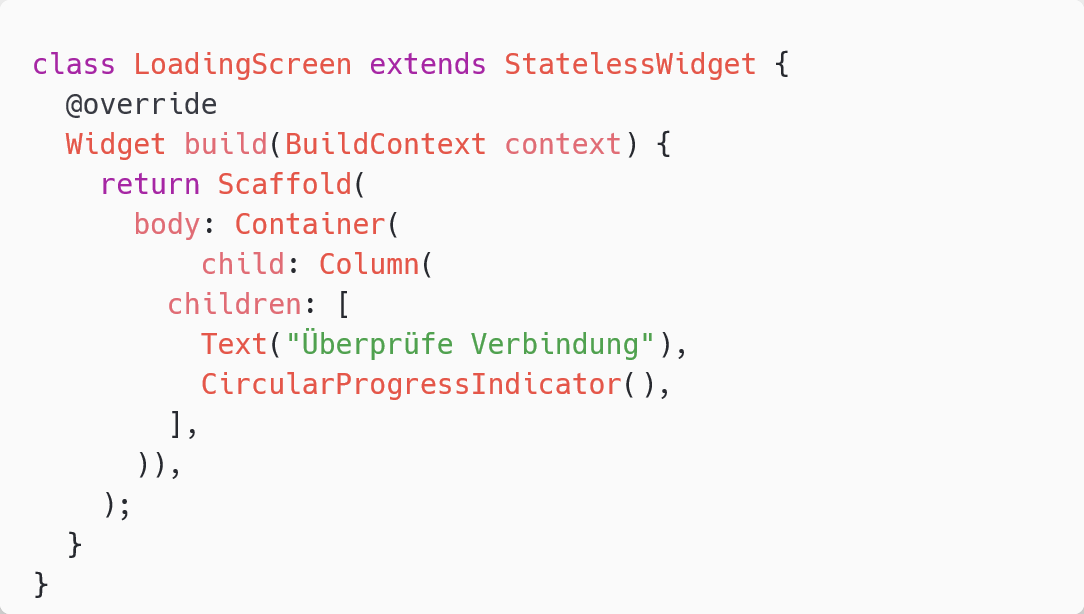
\includegraphics[width=10cm]{images/Theorie/Programmiersprachen/statelessWidget.png}
    \vspace{-25pt}
    \caption{Stateless Widget LoadingScreen welches das eine Ladeseite darstellt}
\end{code}


\subsubsection{Stateful Widget}